\section{Question 5}

\subsection{Question}
\verbatiminput{q5/q5.txt}

\subsection{Answer}

To answer this question, {\tt matrix.py} was modified to add the capability to calculate {\it Term Frequency Inverse Document Frequency (TF/IDF)}. This process normalizes the term frequency against the entire corpus of documents. The added functions for computing TF/IDF are found in Listing \ref{listing:tfidf}. These functions use the master word count dictionary ({\tt wordcounts}) and each blog's individual word count ({\tt wc}) for each of the words in the {\tt wordlist} from Question 1/2.

\lstinputlisting[language=Python, caption={use of tfidf function}, label=listing:tfidf,linerange={116-117},firstnumber=116]{matrix.py}

\lstinputlisting[language=Python, caption={tf idf functions}, label=listing:tfidf,linerange={40-48},firstnumber=40]{matrix.py}

\begin{figure}[h!]
\centering
\fbox{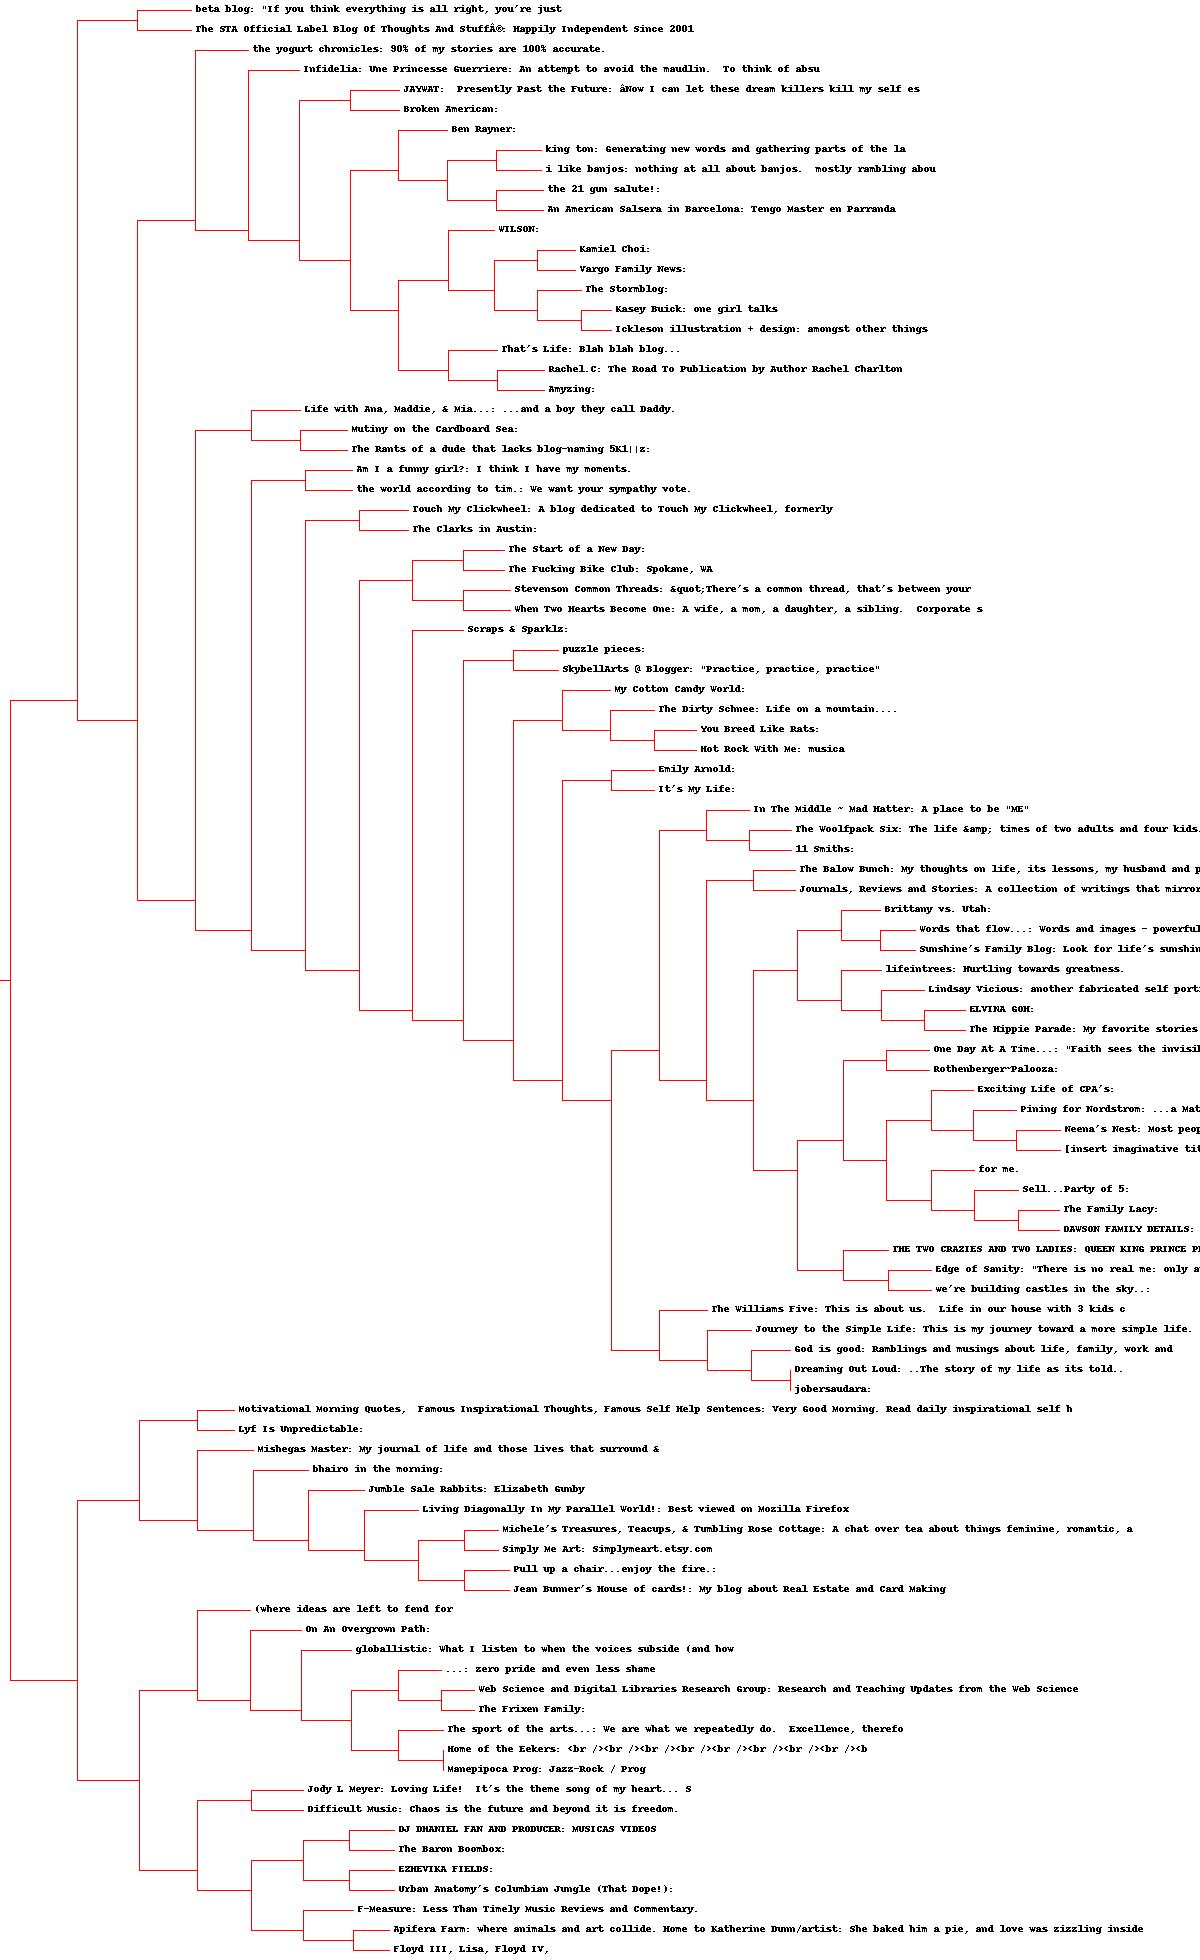
\includegraphics[scale=0.3]{q2/blogclust.jpg}}
\caption{plain count dendrogram}
\label{fig:plain}
\end{figure}

\begin{figure}[h!]
\centering
\fbox{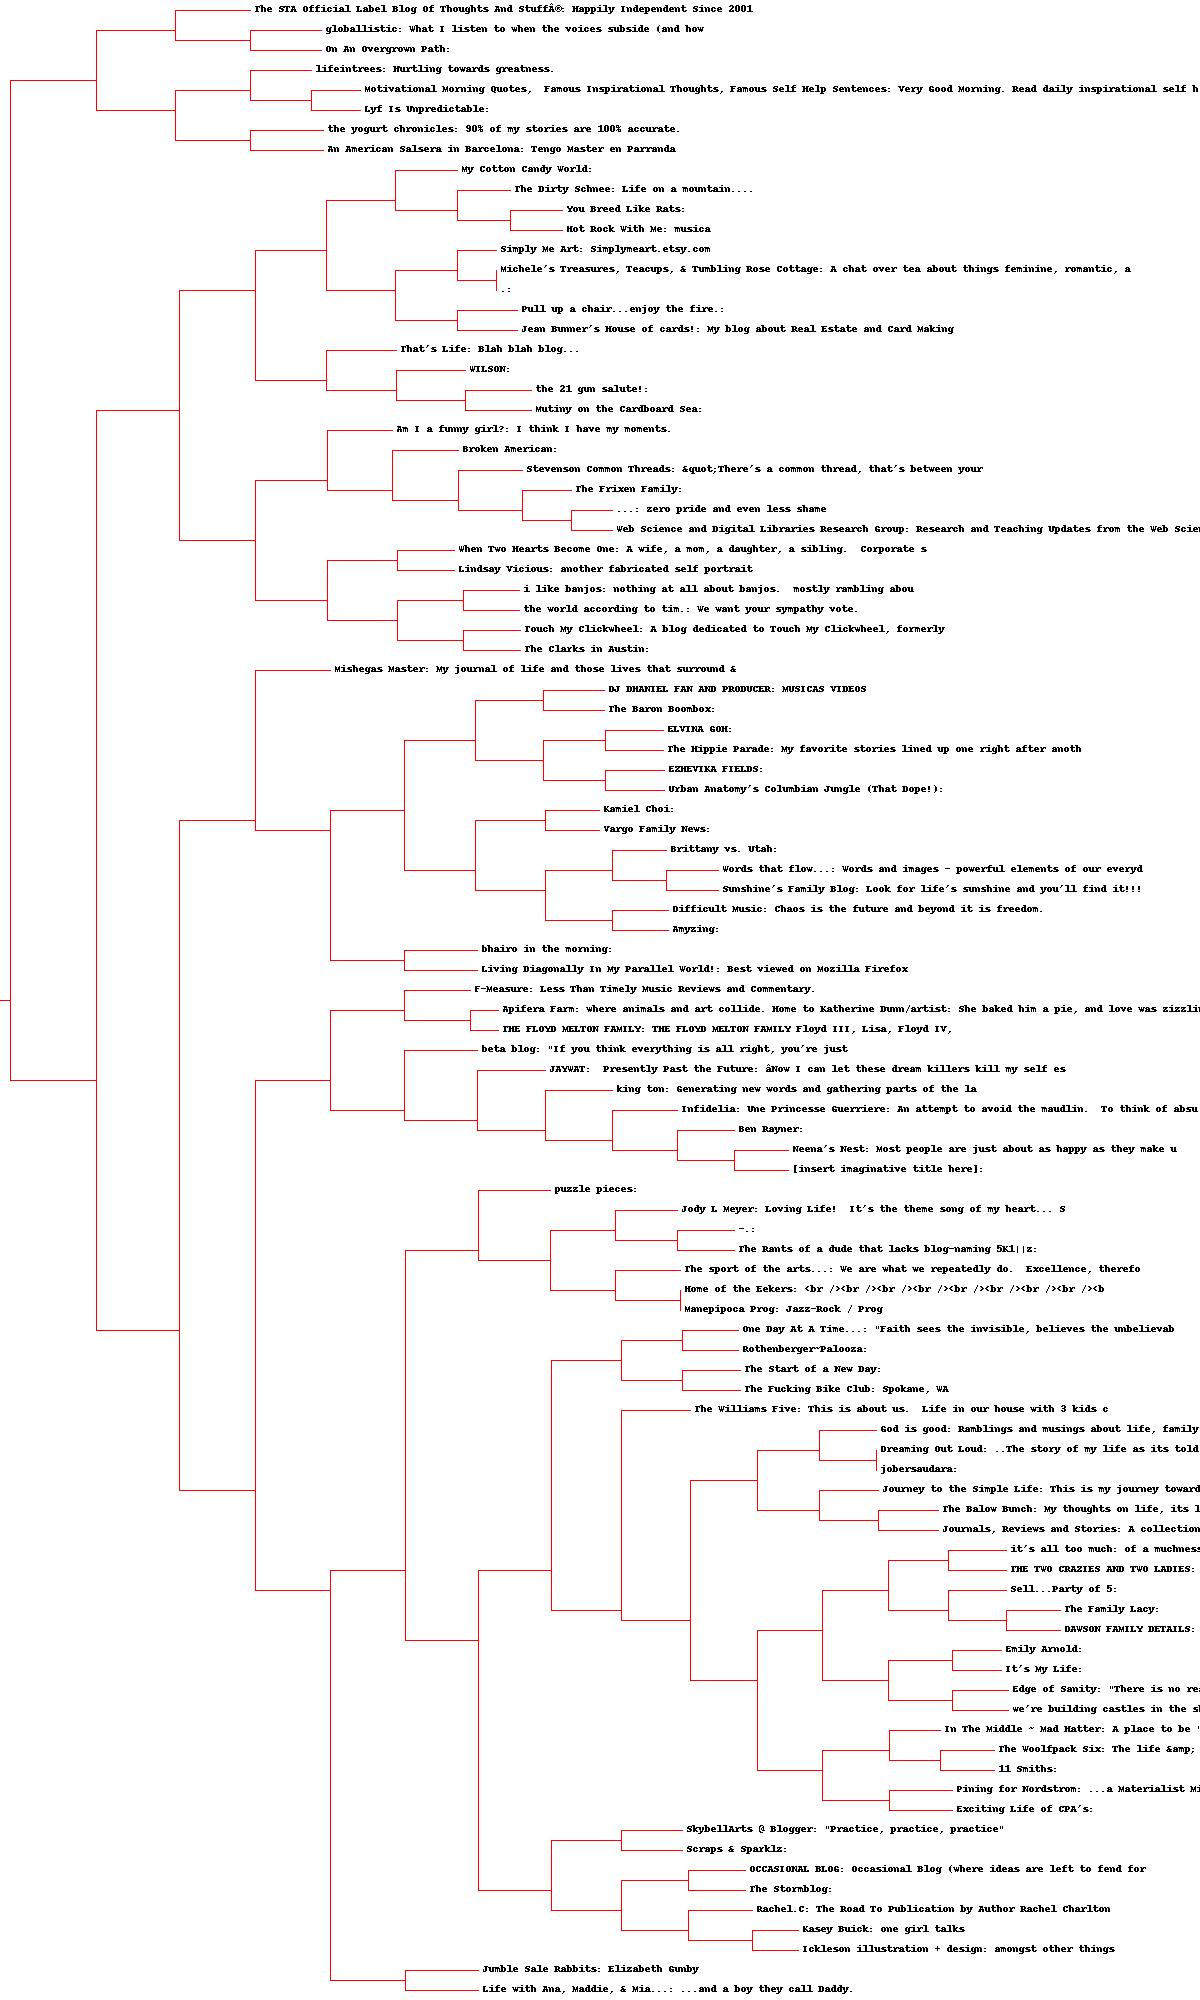
\includegraphics[scale=0.3]{q5/blogclust.jpg}}
\caption{TF/IDF driven dendrogram}
\label{fig:tfidf}
\end{figure}